Här följer en beskrivning över hur de två kurserna samspelar samt lite mer ingående hur de olika VCS fungerar och skillnader mellan dem.
\subsection{Vår situation}

Projektet som vi ska utföra vår studie på är ett delat projekt mellan två kurser. Den ena kursen går ut på att utveckla ett mjukvaruprojekt över en sju veckor lång period. Den andra kursen går ut på att gå in i en ledarroll och coacha en av grupperna under deras projekt. Projektet ska simulera ett verkligt utvecklingsprojekt med en kund och Extreme Programming (XP)~\cite{BeckXP} som utvecklingsmetod. Gruppen kommer att använda sig utav utvecklingsverktyget Eclipse och programmeringen sker i Java. Gruppen har innan projektets början fått lära sig XP och SVN genom föreläsningar och laborationer. För att testa koden under laborationerna kommer JUnit att användas som verktyg.


\subsection{Versionshantering}

I mjukvaruprojekt behöver utvecklarna dela filer och dokument med varandra. I ett mindre projekt med ett fåtal utvecklare går det att komma undan med att skicka filer via email och att tillsammans sitta och sammanfoga dokument. Detta kan med tiden bli mycket tidskrävande och komplicerat med många versioner av samma dokument i omlopp. Det är i ett sådant läge som ett VCS kan användas och förenkla arbetet. Ett VCS tillåter att ett godtyckligt antal utvecklare jobbar med samma projekt och delar alla projektfiler på en plats, även kallat ett repositorie (hädanefter refererat till som repo). När en fil ändras sparas informationen om vad som har ändrats samt att filen får ett nytt versionsnummer. På detta vis håller systemet reda på vilken som är den senaste versionen av en fil samt möjliggör för utvecklarna att återställa en tidigare version av filen.

En ytterligare funktion i VCS är möjligheten att slå samman två versioner av samma fil, även kallat merge. Om flera utvecklare arbetar i samma version av en fil samtidigt och försöker spara den i det gemensamma repot kommer en sammanslagning att behöva göras. Vid enklare ändringar i filen kan ett VCS bidra med att automatiskt slå samman filerna. Däremot om ändringarna är komplicerade eller på samma ställe i filen markerar systemet konflikten och ber utvecklaren att lösa konflikten.

I projekt kan det ibland finnas behov av att utifrån en punkt utveckla systemet parallellt men åt olika håll. Med ett VCS kan man då skapa en förgrening av programmet, även kallad branch. Ett exempel på detta är om utvecklargruppen förbereder för en release av mjukvaran. Då behövs en stabil version av mjukvaran där funktionaliteten är helt färdigställd. För att inte hela projektet ska stanna upp för detta kan man välja att göra en branch när projektet är i ett stabilt läge. Releasearbetarna kan då arbeta på den nya branchen utan risk för att ny, halvfärdig kod följer med i releasen. De andra utvecklarna kan fortsätta att arbeta som tidigare och vid ett senare tillfälle kan man välja att återigen slå ihop branchen med huvudprojektet.


\subsection{CVS/SVN}

\begin{figure}[htb!]\centering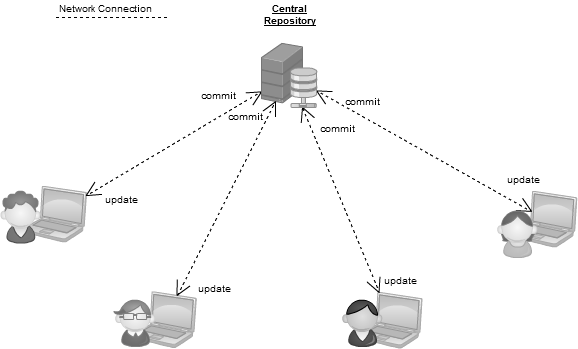
\includegraphics[width=0.75\textwidth]{CVCS.png}\caption{Visar upplägget i ett centraliserat versionshanteringssytem. Alla användare kopplar upp sig mot ett gemensamt repo}\label{fig:CVCSPic}\end{figure}



Datavetenskapsinstitutionen har valt att lära ut ett VCS kallat Concurrent Versions System (CVS) till PVG-projektet. CVS lanserades år 1990 och är ett centraliserat VCS (CVCS). Att det är centraliserat innebär att det har ett centralt repo som alla utvecklare kopplar upp sig mot (se Fig.~\ref{fig:CVCSPic}). I repot finns alla filer samt information om alla ändringar som gjorts. När en utvecklare checkar ut projektet skapas en lokal kopia av det på utveklarens dator. Därefter görs alla ändringar lokalt och när koden är klar laddar utvecklaren upp den i repot och löser eventuella merge-konflikter. Skulle ny kod bli uppladdat på repot går det att göra en uppdatering och på så sätt få de senaste ändringarna i sitt lokala repo. Allt detta kan göras via ett inbyggt användargränssnitt(GUI) i Eclipse. 

	CVS utvecklas inte längre men det finns många CVS-kloner som har samma funktionalitet som CVS. Klonerna är främst utvecklade för att lösa buggar och lägga till funktioner som saknades i den sista släppta versionen av CVS. Subversion (SVN) är en av dessa kloner och är systemet som används under PVG-projekten. Funktionerna som finns i CVS finns även i SVN och fungerar analogt. Även för SVN finns det GUI att installera till Eclipse för att grafiskt hantera projektfilerna. 
 

\subsection{Git}

\begin{figure}[htb!]\centering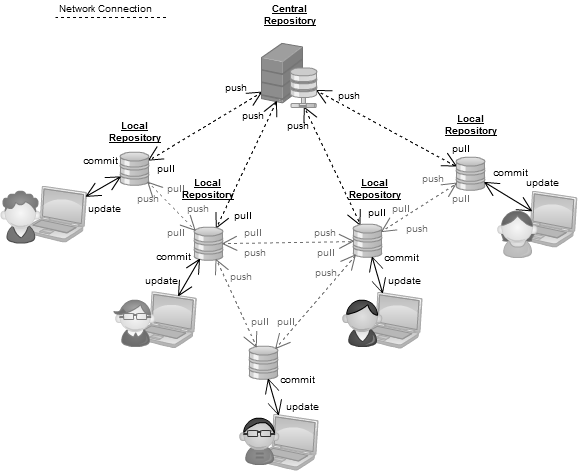
\includegraphics[width=0.75\textwidth]{DVCS.png}\caption{Visar upplägget i ett decentraliserat versionshanteringssytem. Alla användare kan koppla upp sig mot ett centralt repo men kan också dela filer mellan varandra}\label{fig:DVCSPic}\end{figure}


För att hantera källkoden till Linuxkärnan valde Linus Torvalds att utveckla sitt eget system~\cite{Torvalds}. Tidigare hade ett system kallat BitKeeper används men när projektets gratislicens gick ut behövdes ett nytt gratis VCS. Enligt Torvalds kunde inget av de dåvarande gratisalternativen leverera den funktionalitet som behövdes så han valde att istället utveckla sitt eget. Det beslutet resulterade i Git.

Till skillnad från CVS och SVN är Git ett decentraliserat VCS(DVCS). Detta innebär att det inte finns ett gemensamt repo som alla utvecklare använder sig av. Istället delar utvecklarna filerna mellan sig (se Fig. \ref{fig:DVCSPic}). Alla utvecklare har ett eget lokalt repo med alla filer och all filhistorik och när man behöver den senaste versionen av koden hämtar man den från de andra utvecklarna. När en utvecklare själv har gjort ändringar kan han trycka ut den nya koden till de andra utvecklarna. Git kan även användas som ett centraliserat VCS genom att alla hämtar från och trycker upp uppdateringar på en server. En av fördelarna med ett decentraliserat system är att två personer kan arbeta med en del i projektet och dela experimentell kod mellan sig utan att det påverkar resten av teamet. 

	Arbetsflödet i Git påminner mycket om det som används i CVS/SVN. Man arbetar med det lokala repot på samma vis som man arbetar med ett repo i CVS/SVN. Varje gång man gjort ändringar i koden gör man en commit till det lokala repot. När koden är redo att skickas ut till de andra utvecklarna trycker man ut koden till dem, vilket kallas att göra en push. Genom att commita till sitt eget repo får man även lokalt en historik som är enkel att navigera i då man alltid kan återställa filerna till en tidigare commit.
	
	Git kan användas både genom terminaler och genom grafiska GUI. Det finns både plugins och fristående program för att hantera sitt repo. Med installationen av Git medföljer även två simpla GUI som kan användas för att skapa och hantera branchar. Till Eclipse finns pluginet EGit vilket medför att man kan hantera sitt repo inifrån Eclipse.